
The drivetrain of the vehicle is fundamental in the transmission of torque between the wheels and the propeller. A key feature of this type of vehicle and a reason why it functions in the way it does is due to the way the wheels are geared to the propeller. Therefore, for the vehicle to be a valid test model, it must have a well designed, reliable and efficient drivetrain to link to the torque of the wheels to the propeller, and for the gear ratio to be correct to ensure that the propellers RPM is in the desired range for a given ground speed.

The design of the drivetrain is primarily driven by the need to maximise efficiency and ensure limited torque loss between the wheels and propeller. Resistance in the drivetrain directly contributes to vehicle drag which thrust from the propeller must overcome. In minimizing this resistance, producing a positive net thrust on the vehicle becomes more readily achievable. The drivetrain should preferably be simple in design to minimize the number of components, reducing weight which leads to lower rolling resistance and reducing the likelihood of mechanical failures during testing.

\subsection{Design Process and early concepts}

The design process was to consider a range of drivetrain concepts applied to the basic vehicle requirements for a propeller to be mounted to provide thrust, geared to the wheels. The different types of drivetrain system available were considered, and then a concept was developed after selecting the best choice. The drivetrain was designed in close tandem with the structure, due to the need for them to be well integrated. Figures \ref{fig:dtIter1}, \ref{fig:dtIter2} and \ref{fig:dtIter3} show how the vehicle was developed and iterated as further design decisions were made throughout the duration of the project, in response to factors such as availability of parts, cost, simplicity of design, ease of manufacture, and unforeseen problems arising in either manufacture or testing.

The primary design challenge faced for the drivetrain is transmitting torque between 2 shafts (wheel axle and propeller) aligned at 90-degrees to each other. To achieve this, the wheel axle required a 90-degree gearbox to transfer wheel axle torque to an axle either orthogonal or parallel to the propeller shaft above. The secondary challenge of linking this gearbox output to the propeller was then considered. Practical options included using a vertical transmission shaft, chain drive, or belt drive.

\begin{figure}[!htbp]
    \centering
    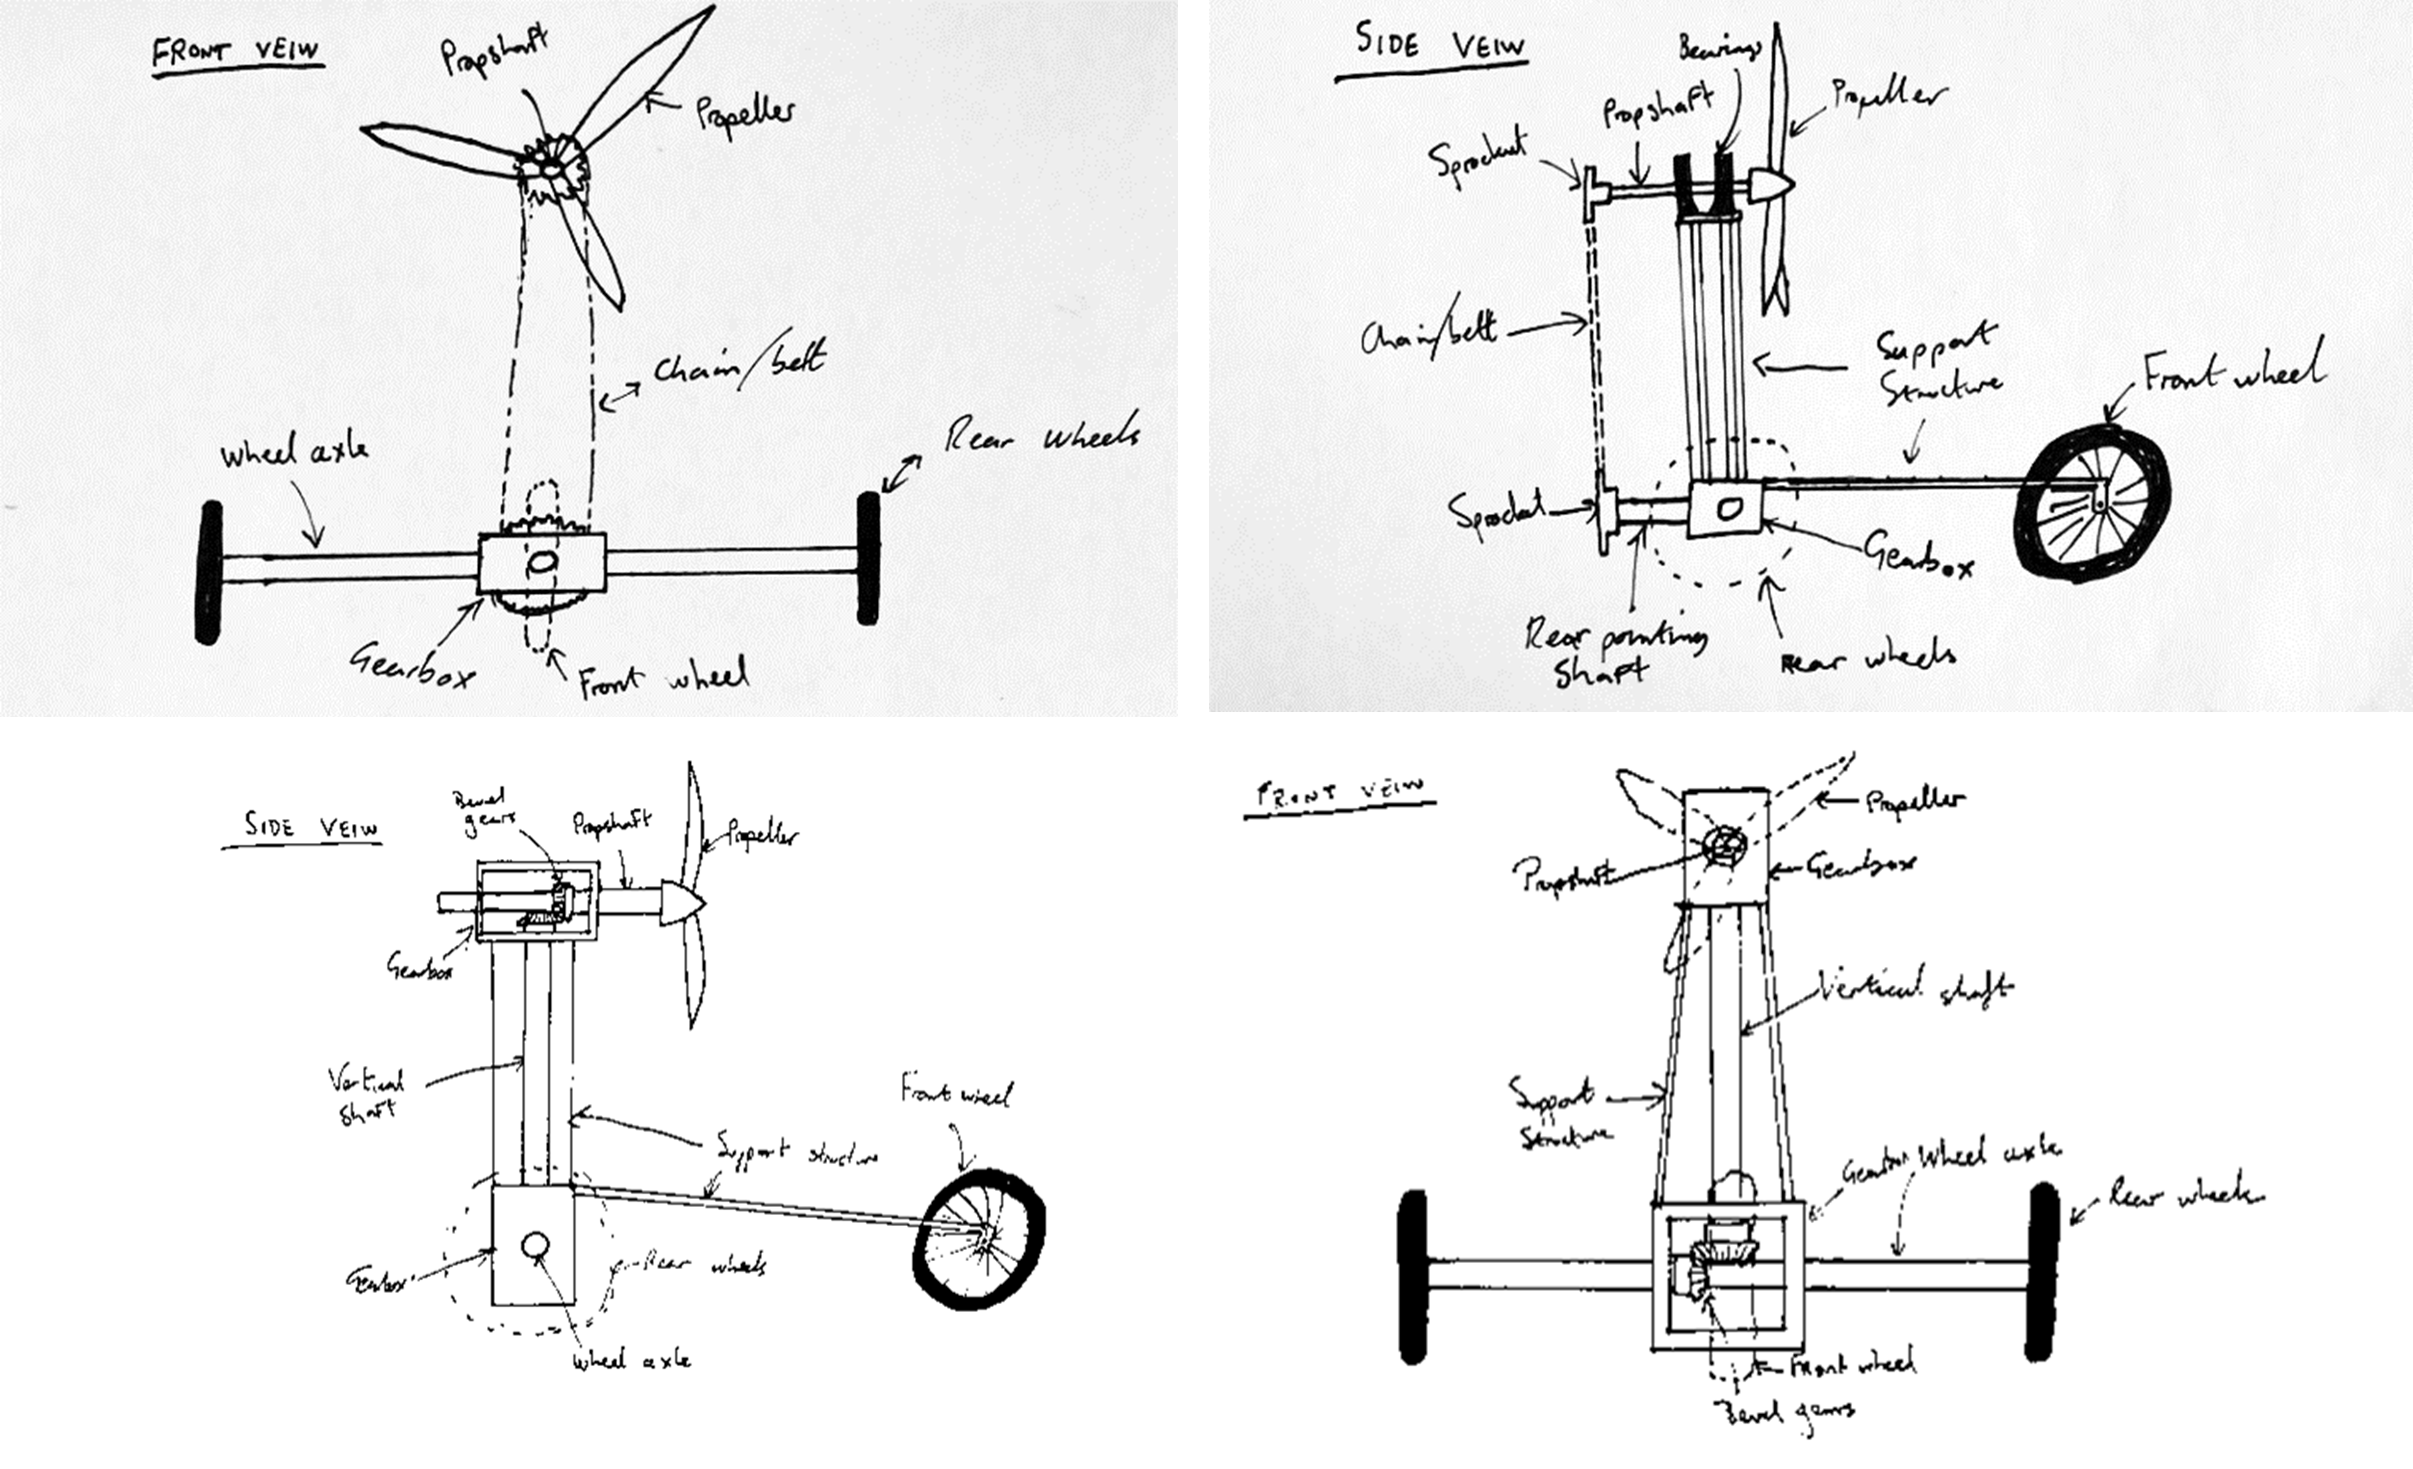
\includegraphics{images/part9/drivetrainSketches.png}
    \caption{Sketches of drivetrain}
    \label{fig:dtsketches}
\end{figure}

% Please add the following required packages to your document preamble:
% \usepackage[table,xcdraw]{xcolor}
% If you use beamer only pass "xcolor=table" option, i.e. \documentclass[xcolor=table]{beamer}
\begin{table}[!htb]
\caption{Drivetrain system choice considerations}
\label{tab:drivetrainChoices}
\centering
\begin{tabular}{|
>{\columncolor[HTML]{\CellColor}}l |p{4cm}|p{4cm}|p{4cm}|}
\hline
\textbf{Type of drivetrain}      & \cellcolor[HTML]{\CellColor}\textbf{Shaft}                                                                                                                       & \cellcolor[HTML]{\CellColor}\textbf{Chain}                                                                     & \cellcolor[HTML]{\CellColor}\textbf{Belt}                                                                                                                    \\ \hline
\textbf{Cost   considerations}   & Shafts come with a cost due to the   amount of material used, often hardened to withstand high torques. Would   require two gearboxes which increases the cost & Chain drive components are cheap with a large range of gear ratios and chain sizes.                        & Belt components are more expensive than chain components. The length of the belt is unchangeable once purchased, assuming the right length can be found. \\ \hline
\textbf{Availability   of parts} & Readily available, variety of   sizes. Limited gearbox options online however                                                                                & Easily acquired, especially for small chain pitches for compact chain drives not coping with high torques. & Rarer than chain parts, difficult to acquire correct sizes.                                                                                              \\ \hline
\textbf{Complexity}              & Simple with minimal interacting   parts                                                                                                                      & Medium complexity, would require tensioner mechanism.                                                      & Would require specialist cogs which run the belt, and a way of applying tension.                                                                         \\ \hline
\textbf{Efficiency}              & High due to small number of   interacting parts, namely 2 bevel gears and shaft bearings on the gearbox                                                      & Losses due to friction between the sprockets and chain.                                                    & Losses due to the elasticity of the belt.                                                                                                                \\ \hline
\textbf{Modularity}              & Only allows for one gear ratio to   be used                                                                                                                  & Allows for sprockets to be changed to alter the gear ratio between tests.                                  & Difficult to adjust or change gear ratios due to high tension.                                                                                           \\ \hline
\textbf{Potential   problems}    & Bevel gears would wear easily if   the shafts were not perfectly aligned, any vibrations could lead to failure   and are difficult to change                 & Vibrations can occur leading to inefficiency and the chain detaching from sprockets during testing.        & The length of the belt is unchangeable once purchased, assuming the right length can be found.                                                           \\ \hline
\end{tabular}
\end{table}

Based on these considerations, the chain drive design was chosen due to the desire to change sprocket sizes and adjust the gear ratio, which can be easily achieved with a chain. Off-the-shelf components for this purpose are less readily available for belt systems. The pure shaft drive would eliminate the possibility of changing gear ratios altogether without a major redesign.
Of all the options, the chain drive design is relatively simple, and the positioning of the two shafts means the chain can be aligned very close to the gearbox and the pylon, reducing stresses in the system when under tension.

\subsection{Chain Tensioner Mechanism}

It was necessary to keep the chain in tension during tests to prevent derailment. This was achieved with a smaller sprocket running on a bearing positioned on a slotted plate about 1/3 of the way up the vehicle A-frame, which could be moved left or right along the slot to apply/remove tension in the chain. A bolt running through the sprocket was used to keep it fixed to the plate.

Figure \ref{fig:tensionerFinal} shows the final chain tensioner mechanism used for the 2nd wind tunnel test. The sprocket has 24-tooth with a bearing custom fitted in the borehole. A series of washers and spacers ensure the sprocket is aligned with the chain, and the two nuts lock the clamping force on the system while the sprocket is allowed to spin freely on the bearing. A secondary safety bolt is fixed in the slot next to the mechanism to prevent tension from releasing during the tests. This final design came about after the first wind tunnel test, which outlined problems with the first design. Initially, as shown in Figure \ref{fig:tensionerInitial}, a 16-tooth sprocket was used, which ran using 3D printed PLA spacers. This worked reasonably well for low ground speed tests, but at ground speeds exceeding 8m/s, the high friction between the sprocket and spacers generated enough heat to soften the PLA (glass transition phase), causing a reduction in clamping force in the tensioner bolt, and loss in the tension of the chain as the tensioner began to move. This led to chain de-railing and potential damage risks to the vehicle/wind tunnel. The 2nd design in Figure \ref{fig:tensionerFinal} eliminated this problem and tension was successfully kept in the chain throughout the tests at all ground speeds after this.

\begin{figure}[!htbp]
    \centering
    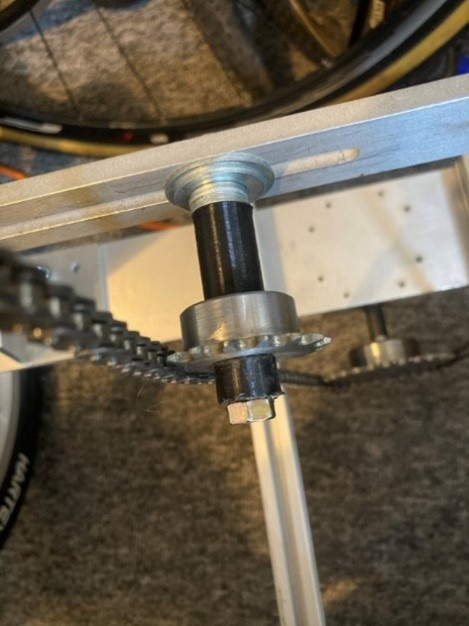
\includegraphics{images/part9/chainTensionerInitial.jpg}
    \caption{Initial chain tensioner mechanism}
    \label{fig:tensionerInitial}
\end{figure}

\begin{figure}[!htbp]
    \centering
    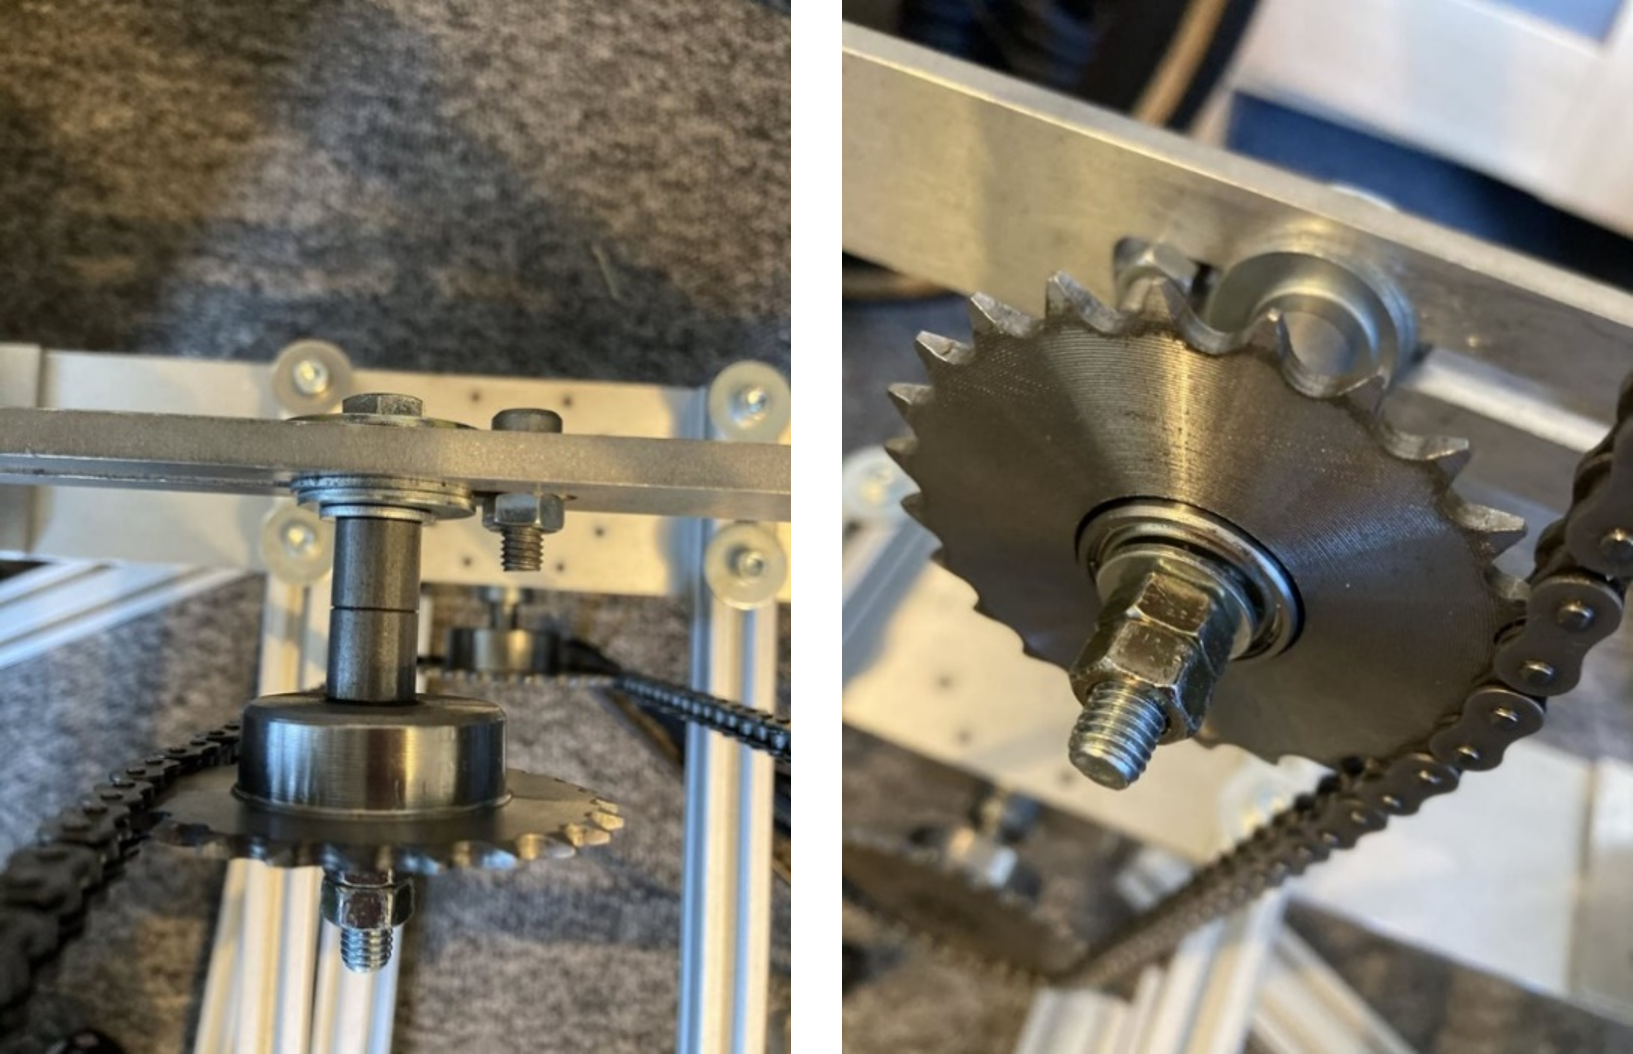
\includegraphics{images/part9/chainTensionerFinal.png}
    \caption{Final chain tensioner mechanism}
    \label{fig:tensionerFinal}
\end{figure}

\subsection{Axle and wheels}

The choice of axle diameter for gearbox input and output was 10 mm. For the torques experienced, it is more than wide enough to limit bending and very unlikely to fail. The initial material choice was hardened stainless steel, which was changed to mild steel due to the need to thread the ends for attachment to the wheels. This was not possible with hardened steel due to its high hardness.

\begin{figure}[!htbp]
    \centering
    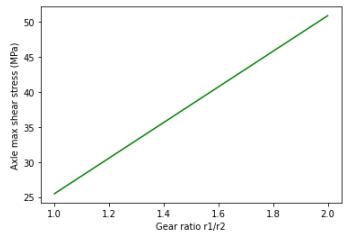
\includegraphics{images/part9/axleStress.png}
    \caption{Maximum shear stress experienced by the rear driven axle as the gear ratio between the sprockets is increased}
    \label{fig:axleStress}
\end{figure}

The maximum shear stress rating for Low Carbon steel is 350 MPa, which is significantly higher than the predicted maximum stresses on the steel axle used on the vehicle. This means the axle has very virtually no risk of failure. The combination of pillow bearings and gearbox bearings pin the axle at various points, evenly distributing the loads from the structure on the axle, which minimises the potential for rotational bending.

\begin{figure}[!htbp]
    \centering
    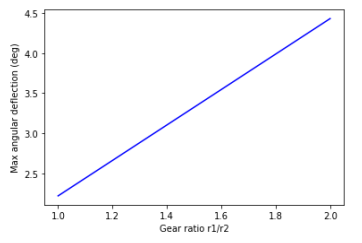
\includegraphics{images/part9/axleDeflection.png}
    \caption{Maximum shear deflection in the axle as gear ratio is increased}
    \label{fig:axleDeflection}
\end{figure}

Figure \ref{fig:axleDeflection} shows the maximum angular deflection for the given maximum torque for each gear ratio is shown. It remains low even at the high gear ratio of 2. This justifies the use of a 10mm steel axle as a lightweight solution, operating well within the parameters in Figures \ref{fig:axleStress} and \ref{fig:axleDeflection}.

The two choices for wheels were metal-spoked bike wheels with a narrow width, for low rolling resistance, or wooden wheels manufactured using laser cut plywood, which would have a rubber band/belt fitted to the circumference to provide traction and damping. Bike wheels with tires containing inner tubes would provide greater damping than the wooden wheels. The decision was made to use off-the-shelf bicycle wheels due to their quality and lightness with a low relative cost. The size of the wheels was determined based on the gear ratio requirements between the angular velocity of the wheels and the propeller.


Figure \ref{fig:propRPM} shows that for a variety of gear ratios, the output RPM of the propeller is not hugely affected by a change in the wheel diameter, ranging here from 14 to 19 inches. Therefore, the choice of wheel size is not hugely driven by the diameter, and a sensible size can be selected based on the vehicle size, market availability and cost considerations.

\begin{figure}[!htbp]
    \centering
    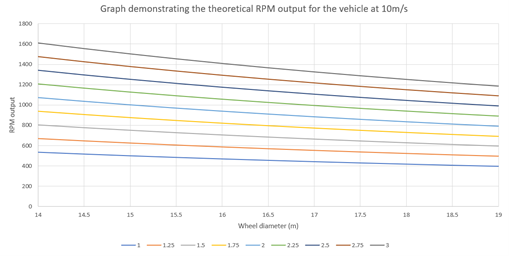
\includegraphics{images/part9/propRPM.png}
    \caption{Propeller RPM vs. wheel diameter for a range of gear ratios}
    \label{fig:propRPM}
\end{figure}

The vehicle was fitted with 16-inch diameter wheels, which were the cheapest and most readily available option. This also was an appropriate size for the wind tunnel, so the load cell wheel mounts could be attached at an appropriate height above the ground, almost level with the wheel hubs. Also, using 16-inch wheels meant the gear ratio used between the two sprockets could be 1:1, as the desired propeller RPM was 470 when the ground speed was 10m/s.

The metal spoked bicycle wheels selected could be easily attached to the 10mm shaft centrally due to the hub design allowing them to be clamped via bolts on the threaded ends of the shaft.

\begin{figure}[!htbp]
    \centering
    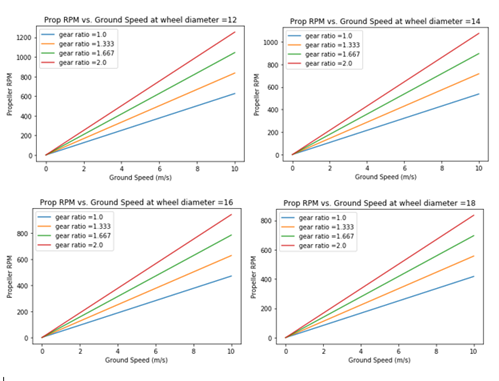
\includegraphics[width = 0.7\linewidth]{images/part9/propRPM2.png}
    \caption{Propeller RPM vs. moving ground speed for a range of gear ratios and wheel diameters (inches)}
    \label{fig:propRPM2}
\end{figure}

Figure \ref{fig:propRPM2} shows that for a wheel diameter of 16 inches, the ground speed of 10m/s, the propeller RPM is 470 when the gear ratio between the lower and upper sprocket is 1, which is the speed to the propeller was designed to operate most effectively at.

Figure \ref{fig:rollResistance} demonstrates how rolling resistance increases with a reduction in wheel radius. With the minimal wheel numbers on the vehicle, the importance of ensuring a minimal rolling resistance can be seen by the large increases in rolling resistances at lower wheel radius values. This was a large consideration when deciding on the wheel radius with the largest diameter possible being selected to minimize this quantity. Furthermore, the 16-inch diameter chosen for the wheels was mainly set by the wind tunnel load cell mounts and their ability to hold the vehicle in place. Reducing the wheel radius from this value was thought to increase the vehicle's rolling resistance, especially with the vehicle size in comparison to the wheels.

\begin{figure}[!htbp]
    \centering
    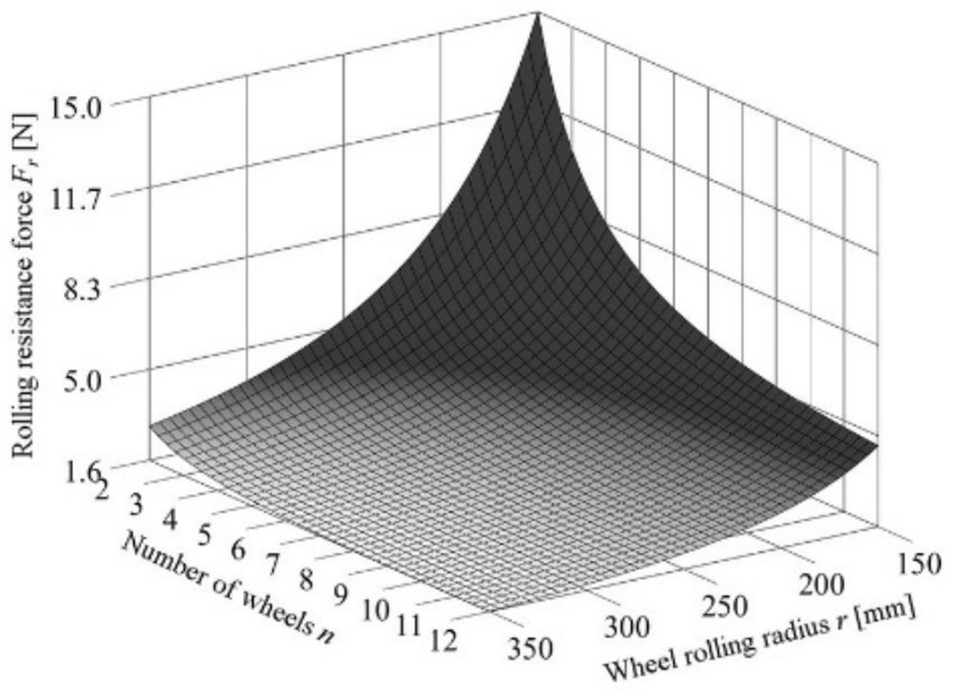
\includegraphics{images/part9/rollingResistance.jpg}
    \caption{Propeller RPM vs. moving ground speed for a range of gear ratios and wheel diameters (inches) \cite{Baldissera}}
    \label{fig:rollResistance}
\end{figure}

\subsection{Gearing and bearings}

A 1:1 gear ratio right angle gearbox was used, which has an aluminium body and stainless-steel bevel gears, which attach via grub screws to 10mm axles aligned at 90-degrees to each other.

For the sprockets, hardened stainless steel Simplex bore sprockets were used, which had an 8mm pitch, so a small, light chain could be used as the torques experienced are low in the drivetrain, with an estimated maximum of 5 Nm.

% Please add the following required packages to your document preamble:
% \usepackage[table,xcdraw]{xcolor}
% If you use beamer only pass "xcolor=table" option, i.e. \documentclass[xcolor=table]{beamer}
\begin{table}[H]
\caption{Gearbox transmission types}
\label{tab:gearboxComp}
\centering
\begin{tabular}{|
>{\columncolor[HTML]{\CellColor}}l |p{6cm}|p{6cm}|}
\hline
\textbf{Gear type}       & \cellcolor[HTML]{\CellColor}\textbf{Advantage}                                                               & \cellcolor[HTML]{\CellColor}\textbf{Disadvantage}                                                          \\ \hline
\textbf{Helical}         & \begin{tabular}[c]{@{}l@{}}Runs smoothly.\\ Can be mounted parallel and straight.\end{tabular}           & \begin{tabular}[c]{@{}l@{}}Must select same handed gears.\\ Power losses due to slippage.\end{tabular} \\ \hline
\textbf{Bevel}           & \begin{tabular}[c]{@{}l@{}}Good slipping resistance.\\ Can easily change a 90 degree angle.\end{tabular} & Prone to noise effects.                                                                                \\ \hline
\textbf{Rack and pinion} & Straight line pitch circle.                                                                              & Rotary to straight line.                                                                               \\ \hline
\textbf{Spiral bevel}    & \begin{tabular}[c]{@{}l@{}}Good noise resistance.\\ Can easily change a 90 degree angle.\end{tabular}    & Prone to slipping.                                                                                     \\ \hline
\end{tabular}
\end{table}

From Table \ref{tab:gearboxComp}, it’s clear to see that the bevel and mitre gearing options were the best two options for gearing the drivetrain gearbox at the centre of the axle rod. The straight-lined bevel gearing is more widely available for general purchase than the mitre option, it was therefore decided that the vehicle would have bevel gears for the gearbox.


% Please add the following required packages to your document preamble:
% \usepackage{multirow}
% \usepackage[table,xcdraw]{xcolor}
% If you use beamer only pass "xcolor=table" option, i.e. \documentclass[xcolor=table]{beamer}
\begin{table}[H]
\caption{Comparison of the different bearing options available}
\label{tab:bearingsComp}
\centering
\begin{tabular}{|m{2.5cm} |l|m{9cm}|}
\hline
\cellcolor[HTML]{\CellColor}\textbf{Type}                    & \cellcolor[HTML]{\CellColor}\textbf{Cost} & \cellcolor[HTML]{\CellColor}\textbf{Additional} \\ \hline
\textbf{Pillow bearing}          &                                       &                                             \\
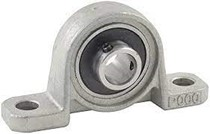
\includegraphics[width=\linewidth]{images/part9/bearing1.jpg}                              & \multirow{-2}{*}{£9.29}               & \multirow{-2}{\linewidth}{Bearing insert aligns with grub screw. Cost effective and light. Comes with clearance holes to increase modularity.}                    \\ \hline
\textbf{Deep grove ball bearing} &                                       &                                             \\
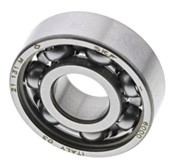
\includegraphics[width=\linewidth]{images/part9/bearing2.jpg}                               & \multirow{-2}{*}{£2.39}               & \multirow{-2}{\linewidth}{Would need welding to a section of the main structure. Cost effective and light.}                     \\ \hline
\textbf{Bolt oval housing}       &                                       &                                             \\
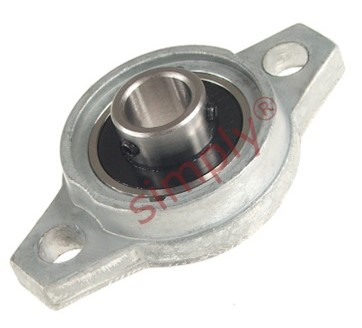
\includegraphics[width=\linewidth]{images/part9/bearing3.jpg}                              & \multirow{-2}{*}{£11.99}              & \multirow{-2}{\linewidth}{Bearing has two grub screws. Clearance holes would allow for modularity in the design. }                     \\ \hline
\end{tabular}
\end{table}

\begin{figure}[!htbp]
    \centering
    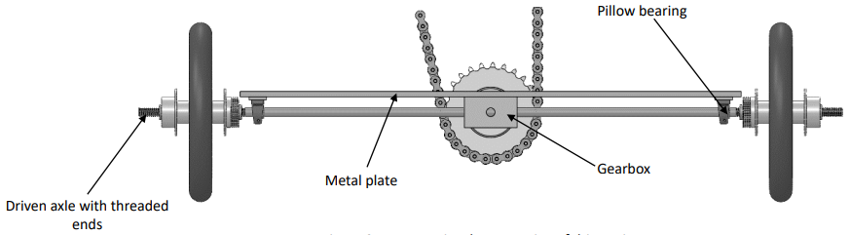
\includegraphics[width=\linewidth]{images/part9/drivetrainbackview.png}
    \caption{Back view of the drivetrain of the vehicle, highlighting the pillow bearing}
    \label{fig:drivetrainBackView}
\end{figure}

The connection between the axle rod and the main horizontal plate for the vehicle illustrated in Figure \ref{fig:drivetrainBackView} had the issue of having one component being in rotation and one component being still on the vehicle. Analysing the different options it was decided that the solution to this issue was using bearings as this would fix the axle rod and maintain the structural integrity of the vehicle. Comparing the different bearing options, Figure \ref{tab:bearingsComp} helped us realise that the pillow block bearing was the best option to complete this connection as this allowed easy connections to be made between the axle rod and the flat plate. The housed bearing offered additional benefits to the vehicle as the guide holes on the components helped increase the vehicle modularity, which would help during the testing of the vehicle if any configuration changes were needed.



